Um professor de matemática que é fascinado por competições resolveu fazer uma
dinâmica com a sua turma. Ele percebeu que em sua casa havia uma grande
quantidade de copos, e optou por utilizá-los em sua próxima aula.

Ele explicou da
seguinte maneira para os seus alunos: Dado $N$ copos ($1 \leq N \leq 10000$), eles
devem determinar qual o maior valor de $B$ tal que é possível formar um
triângulo de base $B$ utilizando no máximo $N$ copos.

Como exemplo, a figura abaixo mostra que, com no máximo $N=8$ copos, é possível formar um
triângulo de base $B=3$:

\begin{center}
    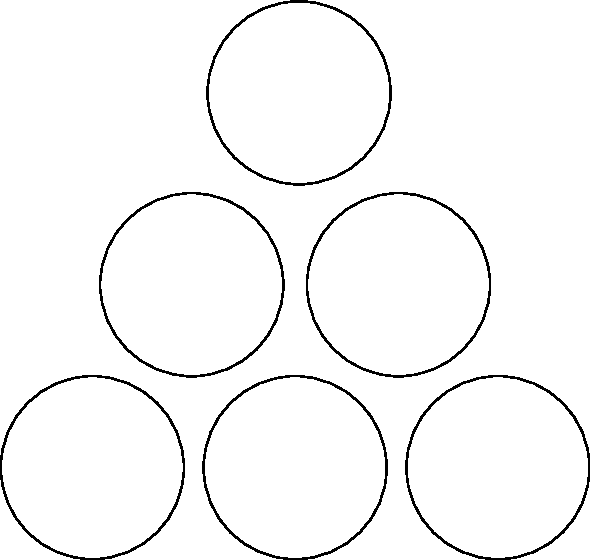
\includegraphics[scale=0.2]{empilha/empilha.pdf}
\end{center}

Neste exemplo, 6 copos são usados e 2 são descartados.

\subsection*{Entrada}

A entrada contém apenas um inteiro $N$ ($1 \leq N \leq 10000$).

\subsection*{Saída}

Imprima o maior valor de $B$ tal que é possível formar um triângulo de base $B$
usando até $N$ copos.

%----- Exemplo 1 -----%
\begin{table}[!h]
\centering
\begin{tabular}{|l|l|}
\hline
\begin{minipage}[t]{3in}
\textbf{Exemplo de entrada}
\begin{verbatim}
10
\end{verbatim}
\vspace{1mm}
\end{minipage}
&
\begin{minipage}[t]{3in}
\textbf{Exemplo de saída}
\begin{verbatim}
4
\end{verbatim}
\vspace{1mm}
\end{minipage} \\
\hline
\end{tabular}
\end{table}

%----- Exemplo 2 -----%
\begin{table}[!h]
\centering
\begin{tabular}{|l|l|}
\hline
\begin{minipage}[t]{3in}
\textbf{Exemplo de entrada}
\begin{verbatim}
8
\end{verbatim}
\vspace{1mm}
\end{minipage}
&
\begin{minipage}[t]{3in}
\textbf{Exemplo de saída}
\begin{verbatim}
3
\end{verbatim}
\vspace{1mm}
\end{minipage} \\
\hline
\end{tabular}
\end{table}

%----- Exemplo 3 -----%
\begin{table}[!h]
\centering
\begin{tabular}{|l|l|}
\hline
\begin{minipage}[t]{3in}
\textbf{Exemplo de entrada}
\begin{verbatim}
1000
\end{verbatim}
\vspace{1mm}
\end{minipage}
&
\begin{minipage}[t]{3in}
\textbf{Exemplo de saída}
\begin{verbatim}
44
\end{verbatim}
\vspace{1mm}
\end{minipage} \\
\hline
\end{tabular}
\end{table}
